\chapter{Evaluating learning algorithm}

\section{Underfitting and overfitting data}
Once the model has been built, we are interested in detecting wheter out model is affected by either \textit{high bias} or \textit{high variance}. In order to better formalize such a concept is interesting to analyze the graph below: 

\begin{figure}[h]
    \centering
    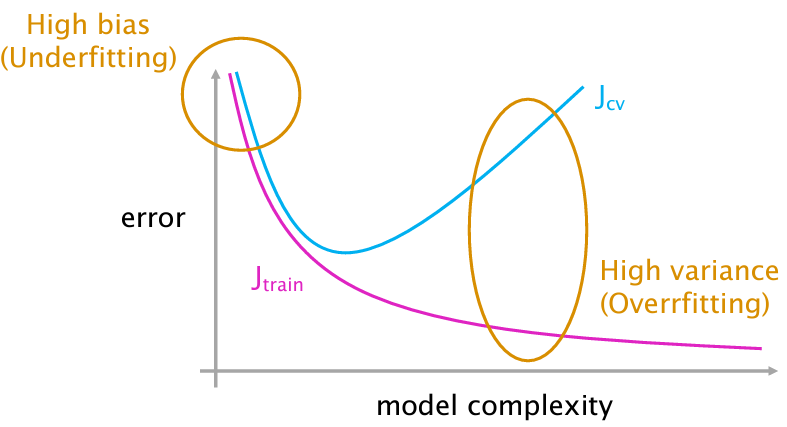
\includegraphics[scale=0.6]{img/bias_variance.png}
    \caption{High-bias vs High-variance}
\end{figure}

\noindent
Only for diagnostic purposes, we collect the data related to the error that the model does on the training data. Clearly the cost function $J_{\text{train}}$ is very high with a  very simple model because the network has not seen a sufficient amount of data. The error on the training set becomes smaller and smaller with the increasing complexity (number of features and so number of parameters of the model). What is very interesting to observe is what happen to the cost function when the validation data are used and the model complexity is growing. At start with a very simple model we have similar cost function, in fact $J_{\text{cv}}$ is very similar to $J_\text{train}$. This situation arises when the model is too simple and the model is \textbf{underfitting the data}. At the opposite when the model complexity grows there is a big difference between the two cost functions. This is related to the fact that the model has very bad performances with never seen data. In this situation we are in front of a problem of \textbf{overfitting the data}: the model has learnt by heart the data, but it is not able to generalize. \\
Both situations must be avoided, as they make a model unusable! The same reasoning can be done by a \textit{different perspective}, that is analyzing what happen to the $J_*$ in function of the dataset size. I have an \textit{high-bias} if at the end of the training phase I have a big error (\textit{with respect  to the human error}). On the other hand, I have an \textit{high-variance} if the model has bad performances on new data, or differently said, the two errors are very different. Note that, both high-variance and bias can be present in some situation. In particular in all cases when the error on training data is high and this is at the same time distant from the cross-validation error.

\begin{figure}[h]
    \centering 
    \subfigure[High-bias]{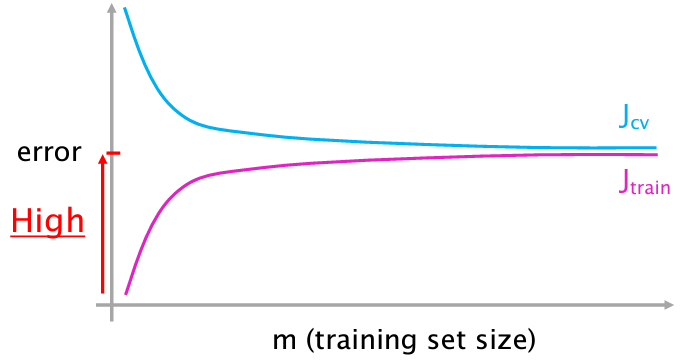
\includegraphics[scale=0.5]{img/bias_variance2.png}}
    \subfigure[High-variance]{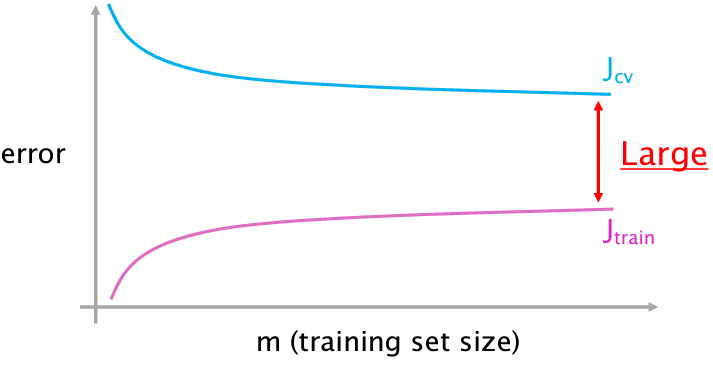
\includegraphics[scale=0.5]{img/bias_variance3.png}} 
\end{figure}

\section{Metrics for model evaluation}
\subsubsection{Motivation}
Given a model which makes a \textit{cancer classification}, suppose we want to evaluate its performance by using the so-called \textbf{accuracy}, we get a 1\% error on the validation/test set. From the labeled data, furthermore, can be analyzed for example that among all the patients only the 0.5\% has cancer. In this case if we take a \textit{Naive classifier} that ignoring the output predicts always $y=0$ (no cancer), such a classifier has better performances than the one we have properly built. The accuracy is not a good metric for evaluating the performance of a machine learning model. In this case the problem appear very evident since the data distribution is \textbf{skewed}. Conclusion: the introduction of other metrics is needed. 

\subsection{Confusion matrix and Precision/Recall}
Especially for classification tasks is useful building a matrix which compare \textit{actual and predicted} values, defining the true/false positive/negative. The one reported below is the so-called \textbf{confusion matrix}:

\begin{figure}[h]
    \centering
    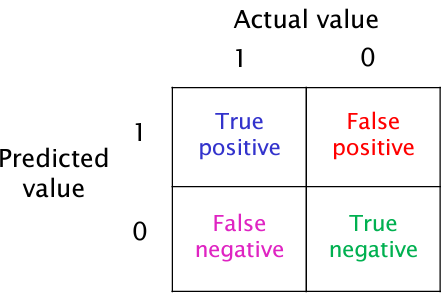
\includegraphics[scale=0.7]{img/confusion.png}
\end{figure}
\noindent
Based on the data collected in such a matrix, we can compute two different metrics: \textbf{precision} and \textbf{recall}. The former answers to the question: "Of all patient we predicted $y=1$, what portion has actually cancer?", the latter "Of all patients where we predicted $y=1$, what portion we did we correctly estimate?". In formulas:
\begin{equation}
    \text{Precision}(p)=\frac{TP}{TP+FP}\quad
    \text{Recall}(r)=\frac{TP}{TP+FN}
\end{equation}
In order to compare such metrics, another auxiliary index is introduced, the $F$ Score which is the armonic mean between recall and precision:
\begin{equation}
    F\text{-score}=\frac{pr}{p+r}
\end{equation}
Other metrics can be used, for example the \textbf{average of the diffenent accuracy indexes} in some situation can make sense, in other different situations also \textit{handcrafted} metrics can be used. It is remarkable that whether we want use eterogeneous metrics it is adviceable to maximize/minimize a single index while having the others as constraints (eg. \textit{maximize \textsf{Accuracy} subject to \textsf{Running time}$\le$100 ns})

\section{Human-level performance}
Sometimes can be useful what is the error that a human do in a classification task in order to understand on what to put the focus (ie. High-bias or high-variance or both), moreover other statistical error-rate can be computed as the \textbf{Bayes Error} which is the \textbf{lowest possible error-rate} for a given classifier. The \textit{Bayes Error} in some situation can be higher with respect to the \textit{Human-error}, this becuse by properly training a neural network the model can have the experience of several humans. Let us give an example:

\begin{figure}[h]
    \centering
    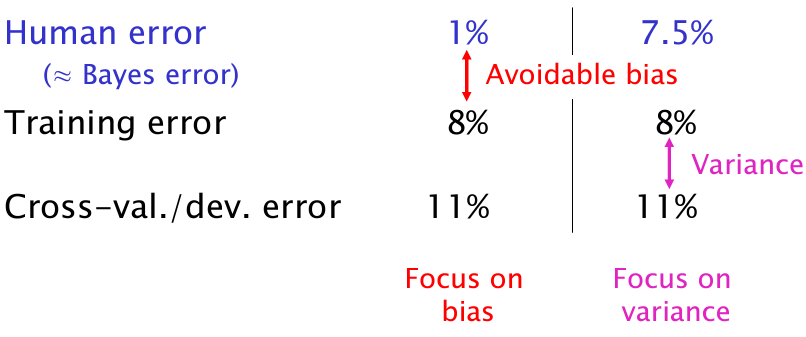
\includegraphics[scale=0.7]{img/performances.png}
\end{figure}
In the first case we can note that there is a bigger difference between the Human and Training error (here is assumed to be very similar to the Bayes error) than the one between training and validation error $\to$ we have to focus ourselves on the bias and use some strategies in order to reduce it. (This is an avoidable bias since it is mostly sufficient making the model grow to eliminate it).\\
In the second case we have similar human and training error, while there is an higher difference between the training and validation error. The most desireable thing is orthogonalize such properties which implies \textbf{having small bias while keeping low variance}, so we want them not to influencing each other (in this  sense \textit{orthogonal}).

\section{Facing bias and variance}
From a study of 2001 it appears evident that:
\begin{quotation}
    "It's not who has the best algorithm that wins, it's who has the most data" (Banko and Brill, 2001)
\end{quotation}
In principle:
\begin{itemize}
    \itemsep-0.2em
    \item In order to \textbf{reduce the bias} could be sufficient to have a \underline{\textbf{bigger model}}; 
    \item In order to \textbf{reduce the variance} could be sufficent to \underline{\textbf{use more data}} in the training phase of the model.
\end{itemize}
From a conceptual point of view it is sufficient to use the following flow-chart:

\begin{figure}[h]
    \centering
    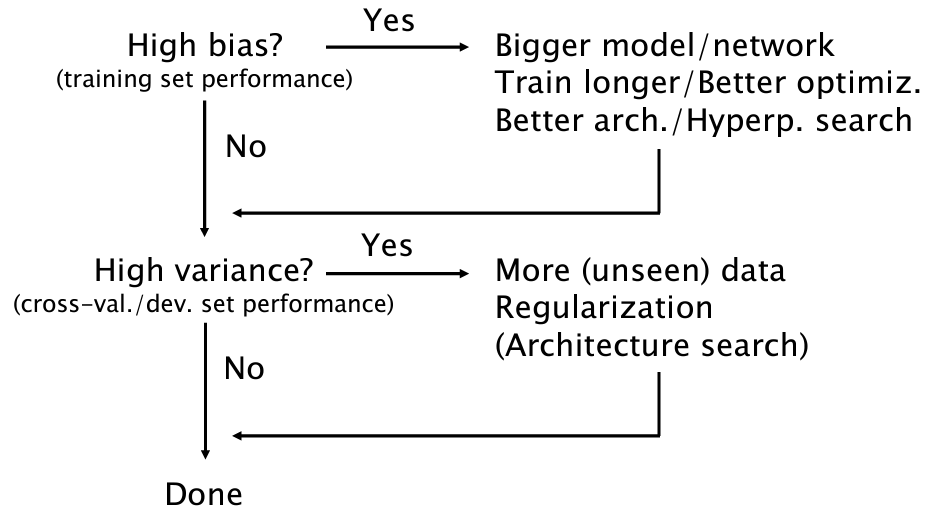
\includegraphics[scale=0.5]{img/flowchart.png}
\end{figure}
\noindent
The real-world examples demonstrates that variance and bias cannot be orthogonalized, then there is a \textbf{trade-off} to manage.

